\chapter{Implementacja programu}
W rozdziale piątym zostały przedstawione najważniejsze fragmenty sposobu implementacji\linebreak programu. Na~początku opisany jest~sposób realizacji detekcji pięciolinii, następnie omawiany jest~proces usuwania wypaczania obrazów. Kolejną częścią jest~opis implementacji modelu uczenia głębokiego oraz~jego niestandardowych klas. w~dalszej kolejności przedstawiony jest~zbiór danych\linebreak GrandStaff, na~którym został wytrenowany model. Rozdział zamyka opis głównej funkcji procesu\linebreak uczenia modelu.

\section{Realizacja detekcji pięciolinii}

Detekcja pięciolinii została opracowana na~podstawie pracy Mariusza Szwocha\cite{Szwoch2005}.

Jedną z~najbardziej przydanych właściwości pięciolinii jest~ich forma, mianowicie pięć prostych, równoodległych linii, co czyni je perfekcyjnymi kandydatami do~detekcji zniekształceń wprowadzonych przez proces fotografowania, pozwalając na~usunięcie niedoskonałości geometrycznych obrazu.

Proces detekcji pozycji pięciolinii na~obrazie został zrealizowany przy pomocy analizy histogramów okienek próbnikowych. Okienkiem próbnikowym nazywany jest~fragment obrazu rozciągający się na~całą jego wysokość i~pewną szerokość, przy pomocy którego dokonywana jest~analiza obrazu, poprzez analizę jego mniejszych fragmentów. Po analizie okienka na~danej części obrazu, jego pozycja jest~przesuwana o~daną odległość w~osi poziomej, po czym następuje analiza następnego wycinka. Poszczególne okienka próbnikowe nie mają na~siebie bezpośredniego wpływu podczas analizy.

\begin{figure}[H]
	\centering
	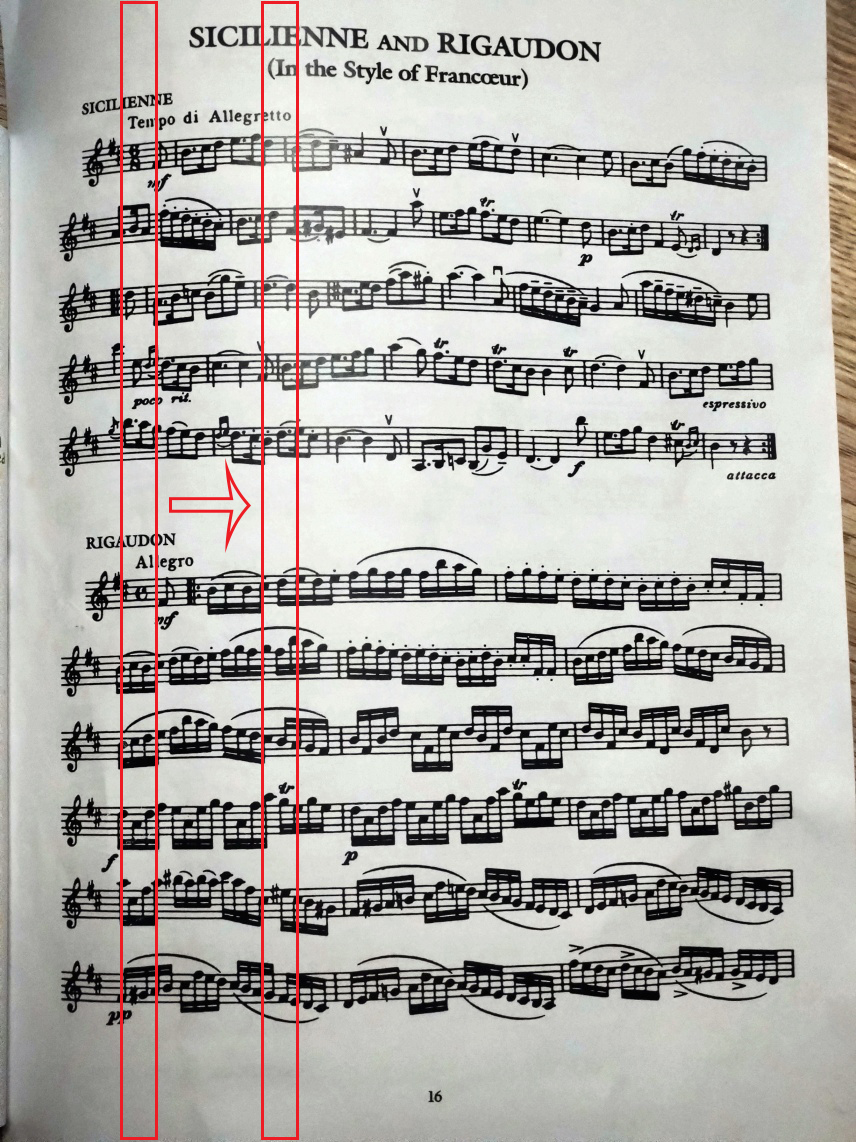
\includegraphics[width=12cm]{images/probe window demo.jpg}
	\caption{Wizualizacja okienka próbnikowego na~zdjęciu nut.}
	\label{fig:probe_window_demo}
\end{figure}

\pagebreak

\subsection{Realizacja detekcji pozycji wypaczonych pięciolinii na~obrazie}

\begin{lstlisting}[caption={\pyth|find_staves_points()| - funkcja odnajdywania pozycji pięciolinii na~obrazie.}, label={find-staves-points}, language=Python]
def find_staves_points(img, img_name, stride = 2):
	img = enhance_image(img, img_name)
	
	img_y, img_x = img.shape[:2]
	
	staff_line_dist = find_staff_line_distance(img)
	if staff_line_dist == -1:
		return -1, 0
	
	staves_positions = find_staves_positions(staff_line_dist, stride, img)
	if len(staves_positions) == 0:
		return -1, -1
	else:
		staves_points_list = make_staves_points_list(staves_positions, staff_line_dist)
		if staves_points_list == -1  or len(staves_points_list) == 0:
			return -1, -1

	return staves_points_list, staff_line_dist
\end{lstlisting}

Powyższa funkcja \pyth|find_staves_points()| jest~odpowiedzialna za~znalezienie i~stworzenie listy punktów, które definiują pozycję pięciolinii. Funkcja ta przyjmuje za~argumenty wczytany obraz, jego nazwę oraz~liczbę kroków. Natomiast zwraca listę zawierającą punkty opisujące położenie pięciolinii oraz~odległość między liniami pięciolinii, albo wartości zawiadamiające kod wywołujący tę funkcję o~wystąpieniu błędu.

Pierwszym krokiem do~poprawnej detekcji pięciolinii na~obrazie jest~uwydatnienie pożądanych jego cech, co jest~wykonywane przy pomocy funkcji \pyth|enchance_image()|, dzięki której możliwa jest~łatwiejsza analiza badanego obrazu. Następnie następuje wywołanie funkcji odpowiedzialnej za~odnalezienie odległości pomiędzy liniami pięciolinii \pyth|find_staff_line_distance()|, poprzez przekazanie obrazu. Jeśli tejże funkcji udało się poprawie odnaleźć szukaną wartość, następuje\linebreak wywołanie kodu mającego odszukać pozycje pięciolinii na~obrazie \pyth|find_staves_positions()| przez przekazanie odnalezionej wcześniej odległości, liczby kroków oraz~obrazu. Kiedy operacja się powiedzie, następuje reformatowanie listy uzyskanych punktów przez funkcję \linebreak \pyth|make_staves_points_list()|, by punkty zawarte w~jednej liście zawierały pozycje pojedynczej pięciolinii. Operacja ta jest~potrzebna, gdyż uzyskane wartości są ułożone w~listach reprezentujących pozycje w~pionowych wycinkach, gdzie~następna część programu będzie potrzebowała ich w~formacie punktów pojedynczej pięciolinii na~jedna listę. w~wypadku powodzenia wszystkich operacji następuje zwrot listy pozycji oraz~odległości pomiędzy liniami pięciolinii.



\subsection{Realizacja uwydatniania obrazu} \label{enhance_image_impl}

\begin{lstlisting} [caption={\pyth|enhance_image()| - funkcja uwydatniania obrazu.}, label={enhance-image}, language=Python]
	def enhance_image(img):
	if len(img.shape) == 3:
		img = cv2.cvtColor(img, cv2.COLOR_RGB2GRAY)
	
	img = cv2.GaussianBlur(img, (5, 5), 0)
	img = cv2.adaptiveThreshold(img, 255, cv2.ADAPTIVE_THRESH_MEAN_C, cv2.THRESH_BINARY, 55, 7)
	
	return img
\end{lstlisting}

Znajdująca się powyżej funkcja ma za~zadanie zmodyfikowanie obrazu, by ten nadawał się do~jego analizy. Odbywa się to przez konwersję obrazu do~odcieni szarości, jeśli jest~on obrazem kolorowym, po czym następuje seria modyfikacji, pozwalających na~uwydatnienie pożądanych \linebreak informacji z~obrazu.

Pierwszą modyfikacją jest~rozmycie gaussowskie, dzięki któremu z~obrazu usuwana jest~część szumu oraz~drobne niedoskonałości są rozmywane, by w~następnym kroku możliwe było lepsze określenie wartości znajdujących się ponad progiem. Kolejną modyfikacją zastosowaną na~obrazie jest~progowanie adaptacyjne, które w~przeciwieństwie do~zwykłego progowania, pozwala\linebreak na~usunięcie cieni z~obrazu, zachowując znajdujące się w~nich dane, które mogą być potrzebne do~poprawnej analizy. Jednocześnie progowanie adaptacyjne automatycznie znajduje odpowiednie wartości progu, dzięki czemu nie istnieje potrzeba określania go ręcznie, co wymaga znaczącej\linebreak ilości czasu i~prób, by~znaleźć taką wartość, która będzie działała w~jak najszerszym zakresie danych wejściowych. Ostatnią modyfikacją dotykającą obraz jest~erozja, która służy do~usunięcia niechcianych punktów i~wyostrzenie linii znajdujących się na~obrazie, co jest~wymagane dla~poprawnego\linebreak odszukiwania pięciolinii.

\newpage

\subsection{Realizacja odnajdywania odległości między liniami pięciolinii} \label{find_staff_line_distance_impl}

\begin{lstlisting} [caption={ \pyth|find_staff_line_distance()| - funkcja odnajdywania odległości między liniami pięciolinii.}, label={find-staff-line-distance}, language=Python]
def find_staff_line_distance(img = np.array):
	img_y, img_x = img.shape[:2]
	probe_window_size = img_x // 40
	probe_window_start_idx = img_x // 5
	probe_window_end_idx = img_x - probe_window_start_idx
	probe_window_hist_arr = np.zeros(img_y)
	staff_line_distance_list = []
	
	for i in range(probe_window_start_idx, probe_window_end_idx, probe_window_size*6):
		make_histogram_array(i, img_y, probe_window_size, img, probe_window_hist_arr)
		peaks_list = filter_out_peaks(probe_window_size, probe_window_hist_arr)
		staff_line_distance = find_staff_line_distance_in_probe(peaks_list)
		
		if staff_line_distance != 0:
			staff_line_distance_list.append(staff_line_distance)
		
		probe_window_hist_arr = np.zeros(img_y)
	
	if len(staff_line_distance_list) != 0:
		return sum(staff_line_distance_list) // len(staff_line_distance_list)
	else:
		return -1
\end{lstlisting}

Umieszczony powyżej kod funkcji \pyth|find_staff_line_distance()| odpowiedzialny jest\linebreak za~odnalezienie odległości pomiędzy liniami pięciolinii na~zdjęciu zapisu nutowego. Funkcja ta\linebreak zaczyna pracę poprzez inicjalizację niezbędnych zmiennych zawierających wartości takie jak: rozmiary obrazu, rozmiar okienka próbnikowego, indeks początkowy poszukiwania, indeks końcowy, tablicę na~której będą przechowywane wartości odczytane z~okienka próbnikowego, oraz~lista potencjalnych\linebreak odległości z~okienek próbnikowych.

Wartości tych zmiennych nie są przypadkowe, szerokość okienka została dobrana eksperymentalnie, podczas to których eksperymentów stwierdzono, iż wielkość równa jednej czterdziestej\linebreak szerokości obrazu daje zadowalające rezultaty, dające poprawne wielkości, natomiast pozycja początkowa i~końcowa okienka próbnikowego gwarantuje, na~poprawnie wykonanych zdjęciach,\linebreak znajdowanie się pięciolinii w~badanym zakresie.

Właściwe odszukiwanie odbywa się iteratywnie poprzez przesuwanie okienka próbnikowego o~wielkości większe od jego szerokości, gdyż nie potrzebujemy analizować całego obrazu, tylko kilka jego fragmentów. Analizowanie pojedynczego okienka może dać niepoprawną wartość odległości, zatem obraz jest~analizowany w~kilku miejscach, by pozyskać właściwą miarę.

W każdym kroku pętli tworzona jest~tablica, na~podstawie której powstaje histogram okienka, dzięki funkcji \pyth|make_histogram_array()|, która zlicza wystąpienia ciemnych pikseli w~każdym\linebreak rzędzie badanego okienka. Następnie z~uzyskanej tablicy, w~funkcji \pyth|filter_out_peaks()|,\linebreak odfiltrowywane są indeksy wysokich wartości histogramu, które powinny być liniami rozpinającymi się na~większość szerokości okienka. na~podstawie uzyskanej listy indeksów w~funkcji\linebreak \pyth|find_staff_line_distance()| odszukiwana jest~odległość między liniami pięciolinii, dzięki\linebreak własności zapisu nutowego, w~którym najczęściej występującą odległością między dwiema liniami w~osi pionowej jest~właśnie odległość pomiędzy składowymi pięciolinii. Jeśli odnaleziona wartość\linebreak nie jest~zerem, to jest~dodawana do~listy potencjalnych odległości. Przed przejściem\linebreak do~następnego kroku pętli, tablica okienka próbnikowego jest~zerowana, by poprzednia analiza\linebreak nie wpływała na~analizę kolejnego okienka.

Gdy analiza okienek się zakończy, jeśli lista potencjalnych odległości nie jest~pusta, zwracana jest~średnia arytmetyczna z~listy odległości w~formie wartości całkowitej, natomiast jeśli lista jest\linebreak pusta, zwracana jest~wartość \textit{-1}, by poinformować kod wywołujący o~błędzie operacji.



\subsection{Realizacja odnajdywania pozycji pięciolinii}

\begin{lstlisting}[caption={\pyth|find_staves_positions()| - funkcja odnajdywania pozycji pięciolinii.}, label={find-staves-positions}, language=Python]
def find_staves_positions(staff_line_distance, stride = 1, img = np.array):
	img_y, img_x = img.shape[:2]
	probe_window_size = (staff_line_distance * 2) + 5
	probe_window_start_idx = probe_window_size * 2
	probe_window_end_idx = img_x - probe_window_start_idx
	probe_window_hist_arr = np.zeros(img_y)
	staves_positions_list = []
	
	for i in range(probe_window_start_idx, probe_window_end_idx, probe_window_size * stride):
		make_histogram_array(i, img_y, probe_window_size, img, probe_window_hist_arr)
		peaks_list = filter_out_peaks(probe_window_size, probe_window_hist_arr)
		staves_positions = get_staves_positions(i, staff_line_distance, peaks_list)
		staves_positions_list.append(staves_positions)
		
		probe_window_hist_arr = np.zeros(img_y)
	
	if len(staves_positions_list) == 0:
		return -1
	else:
		return staves_positions_list
\end{lstlisting}

Odszukiwanie pozycji pięciolinii, realizowane w~funkcji \pyth|find_staves_positions()| odbywa się analogicznie do~działania \pyth|find_staff_line_distance|, z~pewnymi różnicami, mianowicie:
\begin{itemize}
	\item szerokość okienka próbnikowego wynosi dwukrotność odległości między liniami pięciolinii, plus pięć pikseli. Wynika to z~właściwości zapisu nutowego, gdzie~główka nuty jest~nieco szersza, niż odległość między liniami, przez co taka wartość zapewnia, że główka nuty nie będzie\linebreak zajmowała całej szerokości badanej części obrazu, zaburzając odczytywane dane, scalając\linebreak ze~sobą dwie linie.
	\item początkowa pozycja jest~ustalona na~dwie szerokości okienka od lewej krawędzi, końcowa zaś na~dwie szerokości od prawej krawędzi, by uniknąć niepotrzebnej analizy granic obrazu, na~których zazwyczaj nic się nie znajduje, lub~znajdują się tam losowe wartości uzyskane z~tła.
	\item szerokość kroku jest~uzależniona od szerokości okienka oraz~przekazanej wartości kroku, która mówi o~ile okienko ma się przesuwać w~każdym kroku pętli.
	\item po odnalezieniu indeksów dużych wartości histogramu w~każdym korku pętli, wywoływana jest~funkcja \pyth|get_staves_postitions|, która szuka sekwencji, odległych od siebie\linebreak o~wcześniej odszukaną odległość pięciu indeksów na~całej wysokości okienka, tworząc listę punktów z~danego wycinka, na~którym znajdują się pięciolinie. Zwrócona lista jest~dodawana do~listy pozycji na~których zostały wykryte pięciolinie, po czym resetowana jest\linebreak tablica okienka próbnikowego.
\end{itemize}


Gdy analiza okienek się zakończy, jeśli lista pozycji nie jest~pusta, to jest~ona zwracana, natomiast jeśli lista jest~pusta, zwraca się wartość \textit{-1}, by poinformować kod wywołujący o~błędzie operacji.

\newpage

\section{Usuwanie wypaczenia obrazu}

Proces usuwania wypaczenia obrazu jest~dostosowaną pod potrzeby projektu wersją programu opracowanego przez Matta Zuckera\cite{Zucker2016}.

Dzięki rozwojowi uczenia maszynowego, by uzyskać dużą skuteczność odczytywania informacji z~zapisów nutowych, nie jest~wymagane przekształcanie zniekształconego obrazu tak, by pięciolinie posiadały blisko idealnie proste linie, co przy użyciu tradycyjnych metod, jak w~wypadku wertykalnego zapadania. Jednakże wytrenowane modele uczenia maszynowego dalej preferują by dane które\linebreak dostają były jak najbliżej ideału, by były w~stanie jak najdokładniej wydobyć dane. Używany w~tym\linebreak projekcie model został wytrenowany na~danych zawierających pięciolinie zgrupowane klamrą\linebreak (akoladą) po dwie, jednak nie jest~to cała strona zapisana nutami, więc do~jego poprawnego\linebreak działania niezbędna jest~odpowiednia segmentacja danego obrazu na~mniejsze części zrozumiałe dla~modelu, co wymaga, by taki obraz dało się w~poprawny sposób pociąć na~mniejsze tak,\linebreak by nie zawierały niepotrzebnych części innych pięciolinii, do~czego potrzebne jest~właśnie usunięcie wypaczeń obecnych na~zdjęciu.

Z racji tego, że nuty często znajdują się w~folderach, książkach i~innych dokumentach piśmienniczych posiadających usztywniany grzbiet łączący wszystkie jego strony ze~sobą, to bez usuwania\linebreak pojedynczych stron, co często bywa destruktywne, nie da się zrobić takiemu zapisowi zdjęcia,\linebreak na~którym nie byłby on zniekształcony. To, wraz z~potrzebą podzielenia obrazu na~mniejsze kawałki w~odpowiedni sposób powoduje, że krok usuwania wypaczeń jest~niezbędny.

Główną ideą implementacji operacji usuwania wypaczania jest~model parametryczny, w~którym reprezentacja strony jest~określana przez szereg parametrów:

\begin{itemize}
	\item wektor rotacji $r$ i~translacji $t$, oba w~$\mathbb{R}^{3}$, które określają parametry orientacji trójwymiarowej i~pozycję strony
	\item dwa parametry nachylenia $\alpha$ i~$\beta$, które specyfikują zakrzywienie powierzchni
	\item pionowe offsety $y_{1},\ldots,y_{n}$ dla~$n$ poziomych zakresów na~stronie
	\item dla~każdego zakresu $i \in \{1,\ldots,n\}$, poziome offsety $x_{i}^{(1)},\ldots,x_{i}^{(m_{i})}$ dla~$m_{i}$ punktów\linebreak w~horyzontalnej rozpiętości
\end{itemize} 

Trójwymiarowy kształt strony uzyskiwany jest~poprzez przeciągnięcie krzywej przy lokalnej osi~$y$ w~kierunku góra-dół. Każda współrzędna $x$ (lewo-prawo) jest~mapowana do~przemieszczenia $z$\linebreak powierzchni strony. Poziomy przekrój kartki jest~zamodelowany jako kwadratowa funkcja sklejana, której końce są zakotwiczone w~zerze. Kształt tej funkcji może być całkowicie określony przy pomocy jej parametrów $\alpha$ oraz~$\beta$ przy punktach końcowych:

\begin{figure}[h]
	\centering
	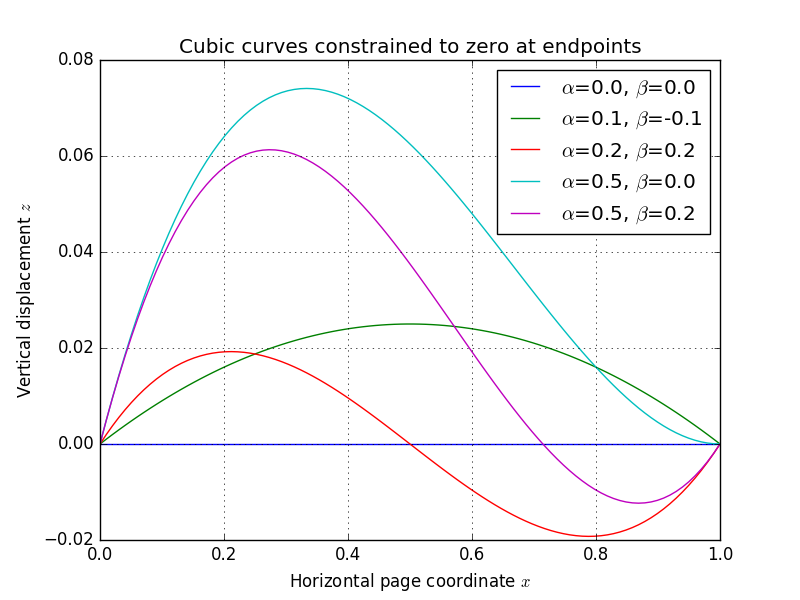
\includegraphics[width=8cm]{images/cubic-splines.png}
	\caption{Przykład kwadratowych funkcji sklejanych z~różnymi parametrami $\alpha$ oraz~$\beta$ z~punktami końcowymi zakotwiczonymi w~zerze. Źródło: https://mzucker.github.io/2016/08/15/page-dewarping.html}
	\label{fig:cubic-splines}
\end{figure}

Jak powyższy wykres pokazuje, zmiany parametrów $\alpha$ oraz~$\beta$ dają nam krzywe, które wyglądają podobnie do~przekroju kartki znajdującej się w~książce.

W momencie kiedy parametry pozycji i~kształtu zostają ustalone, każda współrzędna na~stronie zostaje rzutowana by określić jej położenie na~płaszczyźnie obrazu. Następnie zaczynając z~naiwnego początkowego przypuszczenia, że punkty kluczowe są kolinearne, znajdowane są parametry $r$, $t$, $\alpha$, $\beta$, $y_{1},\ldots,y_{n}$, $x_{i}^{(1)},\ldots,x_{i}^{(m_{i})}$ które minimalizują błąd rzutowania punktów kluczowych.

Po uzyskaniu odpowiedniego modelu, parametry pozycji i~kształtu zostają wyizolowane\linebreak i~następnie używane do~odwrócenia wynikowego mapowania strony na~obraz, by usunąć wypaczenie całego obrazu.




\begin{lstlisting}[caption={\pyth|dewarp_page()| - główna funkcja usuwania wypaczania obrazu.}, label={dewarp-page}, language=Python]
def dewarp_page(img, img_name, staves_positions_in_list):
	shape = img.shape[:2]
	
	staves_positions = get_norm_pos_list(staves_positions_in_list, shape)
	pagemask, page_outline = get_page_extents(img)
	corners, y_coords, x_coords = keypoints_from_samples(pagemask, page_outline, staves_positions)
	rough_dimensions, span_counts, params = get_default_params(corners, y_coords, x_coords)
	destination_points = np.vstack((corners[0].reshape((1, 1, 2)),) + tuple(staves_positions))
	params = optimize_params(destination_points, span_counts, params)
	page_dimensions = get_page_dimensions(corners, rough_dimensions, params)
	dewarped_image = remap_image(img, page_dimensions, params)
	
	return dewarped_image
\end{lstlisting}

Powyższa funkcja \pyth|dewarp_page()| jest~główną funkcją zarządzającą procesem usuwania\linebreak wypaczenia, przyjmuje ona za~argumenty obraz na~którym ma zostać wykonana operacja, jego nazwę oraz~listę zawierającą listy wykrytych pozycji pięciolinii znajdujących się na~obrazie wejściowym.

Rozpoczyna swoje działanie poprzez uzyskanie wymiarów obrazu wejściowego do~zmiennej \linebreak \lstinline|shape|, następnie przechodząc do~przekształcenia listy wykrytych punktów pięciolinii do~postaci norm wektorowych przy pomocy funkcji \pyth|get_norm_pos_list()|.

Kolejnym krokiem jest~pozyskanie punktów kluczowych z~otrzymanych próbek korzystając\linebreak z~funkcji \pyth|keypoints_form_samples()|. Gdy zostaną one określone, przekazywane są one\linebreak do~funkcji \pyth|get_default_params|, by określić domyślne parametry strony, będące założeniem \linebreak iż strona jest~płaska.

Następnie zostaje stworzona tablica punktów docelowych, poprzez wertykalne połączenie punktu reprezentującego lewy górny róg strony i~pozycji wykrytych pięciolinii.

W dalszej kolejności następuje etap optymalizacji otrzymanych parametrów w~funkcji \linebreak\pyth|optimize_params()|, dzięki któremu możliwe jest~określenie prawdziwego kształtu strony przeznaczonej do~usunięcia jej wypaczenia.

Gdy parametry są już zoptymalizowane, pozyskiwane są wymiary strony znajdującej się \linebreak na~obrazie, dzięki funkcji \pyth|get_page_dimentions()|, które są wymagane do~poprawnego\linebreak remapowania obrazu.

Jak program obliczy wszystkie niezbędne parametry do~usunięcia wypaczenia, przechodzi\linebreak do~remapowania obrazu wejściowego w~funkcji \pyth|remap_image()|, z~której uzyskiwany jest~poprawiony obraz, który następnie jest~zwracany do~kodu wywołującego proces usuwania zniekształcenia strony.

\subsection{Realizacja tworzenia punktów kluczowych z~pozyskanych próbek}

\begin{lstlisting}[caption={\pyth|keypoints_from_samples()| - funkcja tworząca tablice punktów kluczowych z~pozyskanych próbek.}, label={keypoints-from-samples}, language=Python]
def keypoints_from_samples(pagemask, page_outline, staff_points):
	all_eigen_vectors = np.array([[0.0, 0.0]])
	all_weights = 0
	
	for points in staff_points:
		_, eigen_vector = cv2.PCACompute(points.reshape((-1, 2)), None, maxComponents=1)
		
		weight = np.linalg.norm(points[-1] - points[0])
		
		all_eigen_vectors += eigen_vector * weight
		all_weights += weight
	
	eigen_vector = all_eigen_vectors / all_weights
	x_dir = eigen_vector.flatten()
	
	if x_dir[0] < 0:
		x_dir = -x_dir
	
	y_dir = np.array([-x_dir[1], x_dir[0]])
	
	pagecoords = cv2.convexHull(page_outline)
	pagecoords = utils.pix2norm(pagemask.shape, pagecoords.reshape((-1, 1, 2)))
	pagecoords = pagecoords.reshape((-1, 2))
	
	px_coords = np.dot(pagecoords, x_dir)
	py_coords = np.dot(pagecoords, y_dir)
	
	px0 = px_coords.min()
	px1 = px_coords.max()
	
	py0 = py_coords.min()
	py1 = py_coords.max()
	
	p00 = px0 * x_dir + py0 * y_dir
	p10 = px1 * x_dir + py0 * y_dir
	p11 = px1 * x_dir + py1 * y_dir
	p01 = px0 * x_dir + py1 * y_dir
	
	corners = np.vstack((p00, p10, p11, p01)).reshape((-1, 1, 2))
	
	ycoords = []
	xcoords = []
	
	for points in staff_points:
		pts = points.reshape((-1, 2))
		px_coords = np.dot(pts, x_dir)
		py_coords = np.dot(pts, y_dir)
		ycoords.append(py_coords.mean() - py0)
		xcoords.append(px_coords - px0)
	
	return corners, np.array(ycoords), xcoords
\end{lstlisting}

Funkcja \pyth|keypoints_form_samples()| ma za~zadanie wyliczenie pozycji rogów oraz~utworzenie tablicy współrzędnych x oraz~tablicy współrzędnych y, na~podstawie otrzymanej maski strony \linebreak i~jej zarysu oraz~listy punktów na~których została wykryta pięciolinia.

Na początku działania funkcja inicjuje dwie zmienne: \pyth|all_eigen_vectors|, będącą zmienną \linebreak mającą przechować wszystkie wektory własne otrzymane z~każdej wykrytej pięciolinii, \linebreak oraz~\pyth|all_weight|, która przechowuje wszystkie wagi z~list pozycji.

Następnie przechodzi ona po wszystkich listach z~listy list punktów pięciolinii znajdujących się na~obrazie, gdzie~oblicza dla~każdej jej wektor własny i~jej wagę, które są dodawane do~wcześniej utworzonych zmiennych pomocniczych.

Po uzyskaniu wszystkich pożądanych wartości, obliczany jest~pojedynczy wektor własny \linebreak dla~całości strony, będący wektorem określającym orientację osi~$x$ \pyth|x_dir|, następnie uzyskiwany jest~wektor orientacji osi~$y$ \pyth|y_dir|.

Kolejnym krokiem jest~pozyskanie współrzędnych strony na~podstawie jej zarysu, poprzez \linebreak utworzenie otoczki wklęsłej, używając funkcji \pyth|convexHull()| z~biblioteki \textit{cv2}, oraz~przetworzenie punktów otoczki na~normy wektorowe.

W dalszej kolejności określane są położenia rogów strony poprzez utworzenie tablicy \pyth|corners|, złożonej z~wektorów określających ich położenie względem zapisu nutowego.

Ostatnim etapem działania tej funkcji jest~stworzenie oddzielnych tablic dla~współrzędnych $x$~i~$y$, które są następnie wypełniane odpowiednio: \pyth|xcoords| współrzędnymi $x$~wszystkich punktów, \linebreak przesuniętych względem skrajnego lewego punktu na~rozważanej stronie, które są produktem \linebreak skalarnym względem odchylenia osi~$x$, \pyth|ycoords| średnią współrzędnych $y$~każdej wykrytej pięciolinii, która jest~przesunięta względem skrajnego górnego punktu rozważanej strony, określone z~produktu skalarnego współrzędnych $y$~punktów wykrytych pięciolinii. 

\subsection{Realizacja ustalania początkowych parametrów modelu}
\begin{lstlisting}[caption={\pyth| get_default_params()| - funkcja tworząca początkowe parametry obrazu.}, label={get-default-params}, language=Python]
def get_default_params(corners, ycoords, xcoords):
	page_width = np.linalg.norm(corners[1] - corners[0])
	page_height = np.linalg.norm(corners[-1] - corners[0])
	rough_dimensions = (page_width, page_height)
	
	span_counts = [len(xc) for xc in xcoords]
	
	cubic_slopes = [0.0, 0.0]
	
	corners_object3d = np.array([
		[0, 0, 0],
		[page_width, 0, 0],
		[page_width, page_height, 0],
		[0, page_height, 0]])
	
	_, roatation_vector, translation_vector = cv2.solvePnP(corners_object3d, corners, CAMERA_MATRIX, np.zeros(5))
	
	params = np.hstack((np.array(roatation_vector).flatten(), np.array(translation_vector).flatten(), np.array(cubic_slopes).flatten(), ycoords.flatten()) + tuple(xcoords))
	
	return rough_dimensions, span_counts, params
\end{lstlisting}

Powyższa funkcja tworzy wstępne parametry obrazu z~wypaczeniem, przyjmując trzy tablice: z~rogami strony, współrzędnymi $y$ oraz~współrzędnymi $x$. Zwraca przybliżone wymiary strony, tablicę zawierającą informacje o~liczebności punktów kluczowych w~każdej wykrytej pięciolinii oraz~tablicę zawierającą wstępne parametry.

Przybliżone wymiary strony uzyskiwane są poprzez obliczenie norm wektorowych z~różnicy \linebreak wektorów, dla~szerokości drugiego i~pierwszego elementu tablicy rogów, dla~wysokości ostatniego i~pierwszego elementu tablicy. 

Tablica liczebności punktów kluczowych w~pięcioliniach jest~tworzona poprzez przejście pętlą \linebreak po tablicy \pyth|xcoords| i~zliczanie długości wewnętrznych tablic w~niej zawartych.

Na parametry składają się wektor rotacji, wektor translacji, tablica parametrów zbocz sklejanej funkcji kwadratowej oraz~wektory współrzędnych. 

Wektory translacji i~rotacji strony uzyskiwane są z~wyniku działania funkcji \pyth|solvePnP|\linebreak(Perspective-n-Point) biblioteki \textit{cv2}, służącej do~obliczania pozycji z~kilku zależności dwuwymiarowych w~przestrzeni trójwymiarowej. Przekazywane do~niej są argumenty wejściowe \linebreak \pyth|corners_object3d|, który jest~założeniem płaskiej strony w~przestrzeni trójwymiarowej,\linebreak \pyth|corners|, zawierający dwuwymiarową, wektorową reprezentację rogów strony, \pyth|CAMERA_MATRIX|, będący macierzą parametrów wewnętrznych kamery, oraz~wektor wejściowy współczynników \linebreak zniekształceń. Gdy wszystkie pożądane wartości zostaną uzyskane, zostają one horyzontalnie złożone do~pojedynczej tablicy, używając funkcji \lstinline|hstack| z~biblioteki \textit{NumPy}.

\newpage

\subsection{Realizacja tworzenia tablicy indeksującej punkty kluczowe}
\begin{lstlisting}[caption={\pyth|make_keypoint_index()| - funkcja tworząca indeksy punktów kluczowych.}, label={make-keypoint-index}, language=Python]
def make_keypoint_index(span_counts):	
	no_of_spans = len(span_counts)
	no_of_points = sum(span_counts)
	keypoint_index = np.zeros((no_of_points+1, 2), dtype=int)
	start = 1
	
	for i, count in enumerate(span_counts):
		end = start + count
		keypoint_index[start:start+end, 1] = 8+i
		start = end
	
	keypoint_index[1:, 0] = np.arange(no_of_points) + 8 + no_of_spans
	
	return keypoint_index
\end{lstlisting}

Zadaniem \pyth|make_keypoint_index()| jest~stworzenie listy indeksującej punkty z~wykrytych \linebreak pięciolinii na~podstawie liczby ich w~konkretnych zakresach zawierających punkty.

Funkcja rozpoczyna działanie inicjując zmienne \pyth|no_of_spans|, przechowującą liczbę wykrytych zakresów zawierających pięciolinie, \pyth|no_of_points|, zawierającą liczbę punktów na~których leżą \linebreak pięciolinie, \pyth|keypoint_index|, dwuwymiarową tablicę rozmiaru $(\text{no\_of\_points} + 1) \times 2$, oraz~zmienną pomocniczą \pyth|start|, zainicjowaną wartością \textit{1}.

Następnie w~pętli for, zaczynając od drugiego elementu, ustawiane są dla~takiej liczby \linebreak pozycji w~liście \pyth|keypoint_index| wartości na~drugiej pozycji każdego edytowanego elementu,\linebreak określające pozycję indeksu współrzędnej $y$ w~liście parametrów, odpowiadającą pozycji na~płaskiej stronie, ile elementów zawiera dana rozpiętość punktów.

Po przejściu pętli, używając funkcji \lstinline|arange| z~biblioteki \textit{NumPy}, ustawiane są na~elementach tablicy \pyth|keypoint_index|, od drugiego elementu w~górę, na~pierwszym miejscu elementów, indeksy współrzędnych $x$ punktów kluczowych.

Uzyskana tablica składa się z~par indeksów punktów kluczowych znajdujących się w~tablicy \linebreak parametrów, przy wstępnym założeniu płaskiej strony.

\newpage

\subsection{Realizacja funkcji rzutującej punkty trójwymiarowe na~płaszczyznę obrazu}

\begin{lstlisting}[caption={\pyth|project_xy()| - funkcja rzutująca punkty obliczonego trójwymiarowego kształtu strony na~płaszczyznę obrazu.}, label={project-xy}, language=Python]
def project_xy(xy_coords, parameter_vector):	
	alpha, beta = tuple(parameter_vector[CUBIC_IDX])
	poly = np.array([ alpha + beta, -2*alpha - beta, alpha, 0])
	
	xy_coords = xy_coords.reshape((-1, 2))
	z_coords = np.polyval(poly, xy_coords[:, 0])
	
	objpoints = np.hstack((xy_coords, z_coords.reshape((-1, 1))))
	
	image_points, _ = cv2.projectPoints(objpoints, parameter_vector[ROTATION_VECTOR_IDX], parameter_vector[TRANSLATION_VECTOR_IDX], CAMERA_MATRIX, np.zeros(5))
	
	return image_points
\end{lstlisting}

Funkcja \pyth|project_xy()| służy do~rzutowania punktów obliczonego trójwymiarowego kształtu strony na~płaszczyznę obrazu.

Zaczyna ona poprzez uzyskanie parametrów $\alpha$ oraz~$\beta$ funkcji sklejanej z~wektora parametrów przekazanego jako argument funkcji, następnie z~pozyskanych wartości tworzy tablicę \pyth|poly| będącą tablicą parametrów wielomianu.

Kolejno następuje przekształcenie tablicy otrzymanych współrzędnych do~pożądanego kształtu. Następnie uzyskiwane są współrzędne $z$ z~wykorzystaniem funkcji \lstinline|polyval()| należącej do~biblioteki \textit{NumPy}, poprzez przekazanie wcześniej utworzonych parametrów wielomianu, oraz~współrzędnych $x$ każdego punktu.

W 8 linii tworzona jest~zmienna \pyth|objpoints| poprzez horyzontalne złączenie tablicy współrzędnych $x$ i~$y$ oraz~wcześniej obliczonych współrzędnych $z$, przekształconych do~pożądanego rozmiaru.

Gdy wszystkie niezbędne dane zostaną obliczone lub~wydobyte, dokonywane jest~rzutowanie punktów z~obliczonymi współrzędnymi w~przestrzeni trójwymiarowej na~dwuwymiarowy obraz\linebreak poprzez wykorzystanie funkcji \pyth|projectPoints()| z~biblioteki \textit{cv2}, która otrzymuje tablicę\linebreak punktów znajdujących się w~układzie współrzędnych świata, wektor rotacji, wektor translacji, macierz\linebreak wewnętrznych parametrów kamery, oraz~wektor parametrów dystorsji. 

Z wyniku rzutowania punktów pozyskiwane są punkty obrazu, które następnie zostają zwrócone.

\newpage

\subsection{Realizacja optymalizacji parametrów modelu}

\begin{lstlisting}[caption={\pyth|optimize_params()| - funkcja optymalizucjąca parametry modelu.}, label={optimize-params}, language=Python]
def optimize_params(destination_points, span_counts, params):
	keypoint_index = make_keypoint_index(span_counts)
	
	def objective(parameter_vector):
		parameter_points = project_keypoints(parameter_vector, keypoint_index)
		return np.sum((destination_points - parameter_points)**2)
	
	result = scipy.optimize.minimize(objective, params, method='Powell')
	params = result.x
	return params
\end{lstlisting}

Powyższa funkcja \pyth|optimize_params()| jest~najważniejszą funkcją całego procesu usuwania\linebreak wypaczania obrazu, w~której odbywa się zasadnicze zminimalizowanie błędu reprojekcji początkowych estymatów pozycji punktów, dzięki któremu możliwe jest~określenie kształtu wypaczonej strony z~zapisem nutowym, które jest~potrzebne by dało się ten proces poprawnie wykonać.

Początkowym krokiem jest~pozyskanie listy indeksującej współrzędne znajdujące się\linebreak w~parametrach przy użyciu funkcji \pyth|make_keypoint_index()|. 

Następnym krokiem jest~zadeklarowanie funkcji wewnętrznej \pyth|objective()|, przyjmującej\linebreak wektor parametrów. Wewnątrz niej następuje stworzenie zmiennej wewnętrznej \pyth|parameter_points| przy użyciu funkcji \pyth|project_keypoints()|, zawierającej listę punktów rzutowanych na~obraz.\linebreak Funkcja ta zwraca kwadrat różnicy punktów docelowych i~punktów rzutowanych linię wyżej.

Główną częścią omawianej funkcji jest~tworzenie zmiennej \pyth|result| przy pomocy optymalizatora z~biblioteki \textit{SciPy}, który dostaje za~argumenty wcześniej utworzoną funkcję wewnętrzną, tablicę\linebreak parametrów oraz~wybierana jest~metoda optymalizacji przy użyciu algorytmu Powella. Dzięki tej\linebreak funkcji wstępne założenia położenia są dopasowywane w~trójwymiarze do~odnalezionych punktów kluczowych na~obrazie, pozwalając na~odnalezienie kształtu, który ma zostać wyprostowany\linebreak do~płaszczyzny. 

Gdy optymalizacja dobiega końca, ze~zmiennej \pyth|result| wyciągane są wartości z~pola \pyth|x|, które następnie zostają zwrócone.

\newpage

\subsection{Realizacja remapowania obrazu}

\begin{lstlisting}[caption={\pyth|remap_image()| - funkcja remapowania wypaczonego obrazu.}, label={remap-image}, language=Python]
def remap_image(img, page_dimensions, params):
	height = 0.5 * page_dimensions[1] * img.shape[0]
	height = utils.round_nearest_multiple(height, REMAP_DECIMATE)
	
	width = utils.round_nearest_multiple(height * page_dimensions[0] / page_dimensions[1], REMAP_DECIMATE)
	
	height_small = height // REMAP_DECIMATE
	width_small = width // REMAP_DECIMATE
	
	page_x_range = np.linspace(0, page_dimensions[0], width_small)
	page_y_range = np.linspace(0, page_dimensions[1], height_small)
	
	page_x_coords, page_y_coords = np.meshgrid(page_x_range, page_y_range)
	
	page_xy_coords = np.hstack((page_x_coords.flatten().reshape((-1, 1)), page_y_coords.flatten().reshape((-1, 1))))
	page_xy_coords = page_xy_coords.astype(np.float32)
	
	image_points = project_xy(page_xy_coords, params)
	image_points = utils.norm2pix(img.shape, image_points, False)
	
	image_x_coords = image_points[:, 0, 0].reshape(page_x_coords.shape)
	image_y_coords = image_points[:, 0, 1].reshape(page_y_coords.shape)
	
	image_x_coords = cv2.resize(image_x_coords, (width, height), interpolation=cv2.INTER_CUBIC)
	image_y_coords = cv2.resize(image_y_coords, (width, height), interpolation=cv2.INTER_CUBIC)
	
	img_gray = cv2.cvtColor(img, cv2.COLOR_RGB2GRAY)
	
	remapped = cv2.remap(img_gray, image_x_coords, image_y_coords, cv2.INTER_CUBIC, None, cv2.BORDER_REPLICATE)
	
	thresh = cv2.adaptiveThreshold(remapped, 255, cv2.ADAPTIVE_THRESH_MEAN_C, cv2.THRESH_BINARY, ADA_THRESH_WIN_SZ, 25)
	
	return thresh
\end{lstlisting}

Powyższa funkcja \pyth|remap_image()| ma za~zadanie, na~podstawie wcześniej określonych parametrów, przemapować obraz wejściowy, co jest~ostatnim krokiem w~usuwaniu wypaczania obrazu, który to jest~bezpośrednią manipulacją obrazu, by to wypaczenie usunąć.

Zaczyna ona swoje działanie poprzez zainicjowanie zmiennej \pyth|height|, przechowującą wysokość obrazu wyjściowego, która jest~uzyskiwana z~połowy wielkości drugiego elementu argumentu \linebreak \pyth|page_dimensions|, pomnożonego przez wysokość obrazu wejściowego, a~następnie zaokrąglonego do~najbliżej wielokrotności 16. Szerokość obrazu wyjściowego jest~uzyskiwana z~najbliżej wielokrotności 16 z~szerokości obrazu wyjściowego, pomnożonego przez stosunek szerokości do~wysokości strony.

Następnie inicjalizowane zmienne \pyth|height_small| oraz~\pyth|width_small|, które są jedną szesnastą odpowiednio: wysokości i~szerokości obrazu wyjściowego.

Kolejno tworzone są tablice \pyth|page_x_range| oraz~\pyth|page_y_range|, wykorzystując funkcję\linebreak \lstinline|linspace()| biblioteki \textit{NumPy}, równoodległych wartości w~zakresie od zera, do~odpowiednio:\linebreak szerokości strony, z~liczbą próbek odpowiadającej \pyth|width_small| oraz~wysokości strony, z~liczbą\linebreak próbek odpowiadającej \pyth|height_small|. z~pomocą tych tablic tworzone są tablice \pyth|page_x_coords| i~\pyth|page_y_coords| korzystając z~funkcji \pyth|meshdrid()| biblioteki \textit{NumPy}, która konstruuje siatkę\linebreak reprezentującą indeksowanie kartezjańskie.

Kolejnym krokiem przygotowującym do~remapowania obrazu jest~stworzenie tablicy \linebreak \pyth|page_xy_coords|, składającej się z~horyzontalnie połączonych ze~sobą i~odpowiednio przekształconych tablic \pyth|page_x_coords| i~\pyth|page_y_coords|, rzutowanych na~typ \textit{float32}.

Dalej tworzona jest~tablica \pyth|image_points|, zawierająca rzutowane punkty obrazu przez funkcję \pyth|project_xy| i~przekształcona z~wartości wektorowych do~pozycji pikseli na~obrazie wejściowym. z~uzyskanych w~ten sposób danych wyciągane są współrzędne $x$ i~$y$ do~zmiennych \pyth|image_x_coords| oraz~\pyth|image_y_coords|, które są przekształcane do~pożądanego kształtu, po~czym zmieniany jest~im rozmiar, by odpowiadały one punktom na~obrazie wyjściowym, wykorzystując funkcję \pyth|resize()| biblioteki \textit{cv2} i~interpolację dwukwadratową.

Gdy już wszystkie niezbędne parametry są określone, tworzony jest~obraz w~skali szarości,\linebreak gdyż informacje o~kolorze nie są potrzebne, po czym następuje zasadnicze przekształcenie obrazu, przy pomocy funkcji biblioteki \textit{cv2} \pyth|remap()|, do~której zostają przekazane jako argumenty: obraz w~skali szarości, mapa współrzędnych $x$, mapa współrzędnych $y$ oraz~flaga interpolacji bikwadratowej oraz~flaga replikacji wartości granicznych obrazu.

\newpage

Po zakończonym remapowaniu, otrzymany obraz jest~progowany adaptacyjnie, by otrzymać\linebreak wartości binarne na~obrazie, bez cieni i~niepotrzebnych do~analizy gradientów. Tak zmodyfikowany obraz pozbawiony wypaczenia jest~zwracany.






\section{Model głębokiego uczenia do~rozpoznawania zapisu nutowego} \label{Model}
Użyty model głębokiego uczenia został opracowany przez Antonio Ríosa-Vilę et. al.\cite{Rios-Vila2023}. 

\begin{lstlisting}[caption={\pyth|E2EScore_CRNN| - klasa modelu głębokiego uczenia do~rozpoznawania zapisu nutowego.}, label={E2E-CRNN}]
class E2EScore_CRNN(nn.Module):

	def __init__(self, in_channels, out_cats):
		super(E2EScore_CRNN, self).__init__()
		self.encoder = Encoder(in_channels=in_channels)		
		self.decoder = RecurrentScoreUnfolding(out_cats=out_cats)
	
	def forward(self, inputs):
		x = self.encoder(inputs)
		x = self.decoder(x)
		return x
\end{lstlisting}

Posiada on architekturę enkoder-dekoder CRNN (ang. \textit{Convolutional Recurent Neural Network}), gdzie~enkoder jest~w~pełni konwolucyjną siecią neuronową, natomiast dekoder jest~rekurencyjną siecią neuronową LSTM (ang. \textit{Long Short-Term Memory}).

Klasa modelu, dziedzicząca po klasie \pyth|Module| biblioteki \textit{PyTorch}, jest~inicjalizowana poprzez podanie do~konstruktora liczby kanałów wejściowych, oraz~liczby kategorii wyjściowych. Wartości tych argumentów są używane by utworzyć obiekty enkodera, któremu podawana jest~liczba kanałów\linebreak wejściowych, oraz~dekodera, reprezentowanego przez klasę \pyth|RecurrentScoreUnfolding|, który\linebreak dostaje liczbę kategorii wyjściowych.

W metodzie \pyth|forward| na~podstawie danych wejściowych tworzona jest~przez enkoder zmienna \pyth|x|, która następnie jest~przekazywana do~dekodera, po czym wynik tej operacji jest~zwracany.

\newpage

\subsection{Realizacja enkodera modelu głębokiego uczenia} \label{Encoder}
\begin{lstlisting}[caption={\pyth|Encoder| - klasa enkodera modelu głębokiego uczenia.}, label={encoder}]
class Encoder(nn.Module):
	
	def __init__(self, in_channels, dropout=0.4):
		super(Encoder, self).__init__()
	
		self.conv_blocks = nn.ModuleList([
			ConvolutionalBlock(in_c=in_channels, out_c=32, stride=(1,1), dropout=dropout),
			ConvolutionalBlock(in_c=32, out_c=64, stride=(2,2), dropout=dropout),
			ConvolutionalBlock(in_c=64, out_c=128, stride=(2,2), dropout=dropout),
			ConvolutionalBlock(in_c=128, out_c=256, stride=(2,2), dropout=dropout),
			ConvolutionalBlock(in_c=256, out_c=512, stride=(2,1), dropout=dropout)
		])
		
		self.dscblocks = nn.ModuleList([
			DSCBlock(in_c=512, out_c=512, stride=(1,1), dropout = dropout),
			DSCBlock(in_c=512, out_c=512, stride=(1,1), dropout = dropout),
			DSCBlock(in_c=512, out_c=512, stride=(1,1), dropout = dropout),
			DSCBlock(in_c=512, out_c=512, stride=(1,1), dropout = dropout)
		])
	
	def forward(self, x):
		for layer in self.conv_blocks:
			x = layer(x)
	
		for layer in self.dscblocks:
			xt = layer(x)
			x = x + xt if x.size() == xt.size() else xt
	
		return x
\end{lstlisting}

\begin{figure}[h]
	\centering
	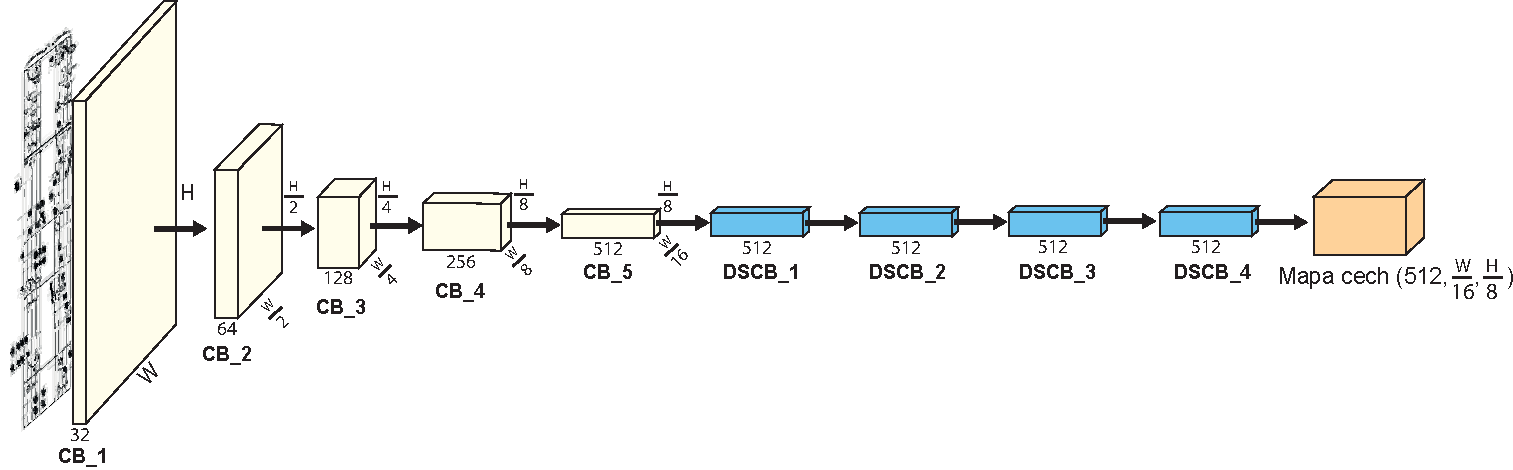
\includegraphics[width=15cm]{images/Encoder_illst.pdf}
	\caption{Wizualizacja struktury enkodera modelu uczenia głębokiego. CB: Blok konwolucyjny, DSCB: Separujący wgłębnie blok konwolucyjny.}
	\label{fig:encoder-model-vis}
\end{figure}

Enkoder, będący klasą dziedziczącą po \pyth|Module| biblioteki \textit{PyTorch}, składa się z~następujących\linebreak po sobie blokach konwolucyjnych, których kanały wyjściowe zwiększają się od 32 do~512, następnie informacje przekazywane są do~następujących po sobie separujących wgłębnie bloków konwolucyjnych (ang. Depthwise Separable Convolution Blocks), których liczba kanałów wejściowych i~wyjściowych zawsze wynosi 512.

Pierwszy blok konwolucyjny posiada krok o~rozmiarze $1 \times 1$, bloki od drugiego do~czwartego $2\times 2$, natomiast ostatni $2 \times 1$. Rozmiar kroku w~przypadku wgłębnych bloków konwolucyjnych jest~dla~nich zawsze taki sam i~wynosi $1 \times 1$.

Dzięki takiej architekturze możliwe jest~przekształcenie wiadomości zawartych na~obrazie tak, by~zamiast zajmować dwuwymiarową przestrzeń, posiadały one formę pojedynczej linii, która jest\linebreak odczytywana jako pojedyncza linijka przez dekoder. Podejście to, nazywane rozwijaniem dokumentu, zostało zaproponowane przez Denisa Coquenet'a, w~pracy dotyczącej wieloliniowego odczytywania pisma odręcznego bez wcześniejszej segmentacji\cite{Coquenet2021}, w~którym model uczy się rozwijać linie tekstu sekwencji od góry do~dołu, by potem je odczytać sekwencyjnie w~ich kolejności czytania. 

Enkoder zaimplementowany w~tym modelu pobiera obraz wejściowy $X \in \mathbb{R}^{C\times H \times W}$ i~zwraca mapę cech $f \in \mathbb{R}^{512, \frac{W}{16}\times\frac{H}{8}}$, gdzie~$C$ oznacza liczbę filtrów używanych przez warstwy konwolucyjne modelu, $W$ szerokość obrazu oraz~$H$ jego wysokość.

Funkcja \pyth|forward()| przechodzi najpierw pętlą przez wszystkie dwuwymiarowe warstwy\linebreak konwolucyjne, podając pierwszej dane wejściowe, zaś każdej kolejnej przekazując zmodyfikowane dane przez warstwę poprzednią. Następnie w~pętli przechodzi ona po wszystkich warstwach separujących wgłębnie sieci konwolucyjnych, gdzie~w~każdym kroku pętli wynik działania warstwy jest\linebreak dodawany do~wcześniejszego, o~ile ich rozmiary są sobie równe, jeśli nie, to zmienna \pyth|x| jest~ustalana jedynie na~wynik działania warstwy. Gdy dane wejściowe przejdą przez obie pętle, zostają zwrócone.

\newpage

\subsubsection{Realizacja bloku konwolucyjnego} \label{ConvBlock}
\begin{lstlisting}[caption={\pyth|ConvolutionalBlock| - klasa bloku konwolucyjnego.}, label={convblock}]
class ConvolutionalBlock(nn.Module):
def __init__(self, in_c, out_c, stride=(1,1), kernel=3, activation=nn.ReLU, dropout=0.4):
	super(ConvolutionalBlock, self).__init__()
		self.activation = activation()
		self.conv1 = nn.Conv2d(in_channels=in_c, out_channels=out_c, kernel_size=kernel, padding=kernel//2)
		self.conv2 = nn.Conv2d(in_channels=out_c, out_channels=out_c, kernel_size=kernel, padding=kernel//2)
		self.conv3 = nn.Conv2d(in_channels=out_c, out_channels=out_c, kernel_size=(3,3), padding=(1,1), stride=stride)
		self.normLayer = nn.InstanceNorm2d(num_features=out_c, eps=0.001, momentum=0.99, track_running_stats=False)
		self.dropout = MixDropout(dropout_prob=dropout, dropout_2d_prob=dropout/2)
	
	def forward(self, inputs):
		pos = random.randint(1,3)
		
		x = self.conv1(inputs)
		x = self.activation(x)
		
		if pos == 1:
			x = self.dropout(x)
		
		x = self.conv2(x)
		x = self.activation(x)
		
		if pos == 2:
			x = self.dropout(x)
		
		x = self.normLayer(x)
		x = self.conv3(x)
		x = self.activation(x)
		
		if pos == 3:
			x = self.dropout(x)
		
		return x
\end{lstlisting}

Klasa bloku konwolucyjnego składa się z~funkcji aktywacji, będącą funkcją klasy bazowej \pyth|Module| biblioteki \textit{PyTorch}, trzech dwuwymiarowych warstw konwolucyjnych, gdzie~pierwsza i~druga\linebreak posiadają rozmiar jądra jak przekazany przy inicjalizacji klasy, oraz~padding wielkości wartości\linebreak całkowitej połowy jądra, zaś trzecia warstwa ma ustawiony rozmiar jądra na~$3\times 3$ i~padding na~$1 \times 1$ oraz~jako jedyna ma ustawiany krok na~wielkość przekazaną jako argument konstruktora. Kolejną\linebreak warstwą tego bloku jest~warstwa normalizacji instancji, inicjowana liczbą cech równą wielkości kanałów wyjściowych, $\epsilon = 0.001$ oraz~momentem równym $0.99$. Ostatnią inicjowaną warstwą jest\linebreak usuwanie mieszane, z~argumentami prawdopodobieństwa usunięcia równym \pyth|dropout| i~prawdopodobieństwem dwuwymiarowego usunięcia równym połowie \pyth|dropout|.

Metoda \pyth|forward| na~początku swojego działania losuje liczbę całkowitą z~zakresu $<1, 3>$,\linebreak używaną do~losowego określenia położenia w~łańcuchu wydarzeń, za~którą aktywacją dwuwymiarowych warstw konwolucyjnych następuje wywołanie \pyth|droput|.

Następnie przekazuje dane wejściowe do~pierwszej warstwy konwolucyjnej, po której następuje aktywacja, druga warstwa otrzymuje jako dane wejściowe wyjście warstwy pierwszej, gdzie~po~niej również następuje aktywacja. Przed trzecią warstwą konwolucji wykonywana jest~normalizacja\linebreak instancji, której wynik jest~przekazywany trzeciej warstwie, po której również następuje aktywacja. Gdy dane wejściowe przejdą przez ten proces, zostają one zwrócone. 


\subsubsection{Realizacja separującego wgłębnie bloku konwolucyjnego} \label{DSCBlock}
\begin{lstlisting}[caption={\pyth|DSCBlock| - klasa głębokiego separującego bloku konwolucyjnego.}, label={dscblock}]
class DSCBlock(nn.Module):

	def __init__(self, in_c, out_c, stride=(2, 1), activation=nn.ReLU, dropout=0.4):
		super(DSCBlock, self).__init__()
		
		self.activation = activation()
		self.conv1 = DepthSepConv2D(in_c, out_c, kernel_size=(3, 3))
		self.conv2 = DepthSepConv2D(out_c, out_c, kernel_size=(3, 3))
		self.conv3 = DepthSepConv2D(out_c, out_c, kernel_size=(3, 3), stride=stride)
		self.norm_layer = nn.InstanceNorm2d(num_features=out_c, eps=0.001, momentum=0.99, track_running_stats=False)
		self.dropout = MixDropout(dropout_prob=dropout, dropout_2d_prob=dropout/2)
	
	def forward(self, x):
		pos = random.randint(1, 3)
		
		x = self.conv1(x)
		x = self.activation(x)
		
		if pos == 1:
			x = self.dropout(x)
		
		x = self.conv2(x)
		x = self.activation(x)
		
		if pos == 2:
			x = self.dropout(x)
		
		x = self.norm_layer(x)
		x = self.conv3(x)
		
		if pos == 3:
			x = self.dropout(x)
		
		return x
\end{lstlisting}

Klasa separującego wgłębnie bloku konwolucyjnego składa się z~funkcji aktywacji, będącą\linebreak funkcją klasy bazowej \pyth|Module| biblioteki \textit{PyTorch}, trzech dwuwymiarowych wgłębnie separujących warstw konwolucyjnych, każda posiadająca jądro wielkości $3 \times 3$, natomiast tylko trzecia warstwa ma\linebreak ustawiony odmienny rozmiar kroku, który zamiast domyślnego rozmiaru $1 \times 1$ posiada wielkość $2 \times 1$. Kolejnym elementem składowym jest~warstwa normalizacji instancji, inicjowana liczbą cech równą wielkości kanałów wyjściowych, $\epsilon = 0.001$ oraz~momentem wynoszącym $0.99$, natomiast\linebreak ostatnią inicjowaną warstwą jest~mieszane usuwanie, z~argumentami prawdopodobieństwa\linebreak usunięcia równym \pyth|dropout| i~prawdopodobieństwem dwuwymiarowego usunięcia równym\linebreak połowie \pyth|dropout|.

Metoda \pyth|forward()| na~początku działania losuje po której warstwie konwolucji zostanie\linebreak wykonane mieszane usuwanie, następnie dane wejściowe przekazywane są pierwszej warstwie\linebreak konwolucji, po której następuje aktywacja, podobnie dzieje się z~warstwą drugą, natomiast przed trzecią konwolucją dokonywana jest~normalizacja instancji, dopiero po której przekazuje się dane przez nią przetworzone do~następnej warstwy, po której nie następuje, w~przeciwieństwie do~warstw poprzednich, aktywacja. Tak przetworzone dane następnie zostają zwrócone.



\subsubsection{Realizacja usuwania mieszanego}

\begin{lstlisting}[caption={\pyth|MixDroput| - klasa usuwania mieszanego.}, label={mix-dropout}]
class MixDropout(nn.Module):
	def __init__(self, dropout_prob=0.4, dropout_2d_prob=0.2):
		super(MixDropout, self).__init__()
		
		self.dropout = nn.Dropout(dropout_prob)
		self.dropout2D = nn.Dropout2d(dropout_2d_prob)
	
	def forward(self, inputs):
		if random.random() < 0.5:
			return self.dropout(inputs)
		return self.dropout2D(inputs)
\end{lstlisting}

By zapobiec nadmiernego dopasowania modelu uczenia maszynowego, ważne jest~używanie w~jego konstrukcji funkcji zerujących niektóre węzły modelu, gdzie~w~przedstawianym modelu zostało to zrealizowane w~sposób mieszany, określany losowo co do~zastosowanej metody przy każdym wywołaniu.

Klasa usuwania mieszanego jest~inicjalizowana w~konstruktorze poprzez podanie prawdopodobieństwa usunięcia węzłów oraz~dwuwymiarowego prawdopodobieństwa usunięcia węzłów, które są przekazywane tworzonym obiektom odpowiadającym im klas \pyth|Dropout| oraz~\pyth|Dropout2d|\linebreak biblioteki \textit{PyTorch}.

W funkcji \pyth|forward| losowo określane jest, z~równym prawdopodobieństwem, czy nastąpi\linebreak zerowanie losowych elementów poprzez wywołanie \pyth|dropout|, czy losowe zerowanie całych kanałów tensora wejściowego przy użyciu \pyth|dropout2D|. Wynik działania jest~następnie zwracany. 


\subsubsection{Realizacja wgłębnie separującej konwolucji}

\begin{lstlisting}[caption={\pyth|DepSepConv2D| - klasa wgłębnie separującej konwolucji dwuwymiarowej.}, label={DepSepConv}]
class DepthSepConv2D(nn.Module):
	def __init__(self, in_channels, out_channels, kernel_size, activation=None, padding=True, stride=(1,1), dilation=(1,1)):
		super(DepthSepConv2D, self).__init__()
	
		self.padding = None
		
		padding = [int((k-1)/2) for k in kernel_size]
		
		if kernel_size[0] % 2 == 0 or kernel_size[1] % 2 == 0:
			padding_h = kernel_size[1] - 1
			padding_w = kernel_size[0] - 1
			self.padding = [padding_h//2, padding_h-padding_h//2, padding_w//2, padding_w-padding_w//2]
			padding = (0, 0)
		
		self.depth_conv = nn.Conv2d(in_channels=in_channels, out_channels=in_channels, kernel_size=kernel_size, dilation=dilation, stride=stride, padding=padding, groups=in_channels)
		self.point_conv = nn.Conv2d(in_channels=in_channels, out_channels=out_channels, dilation=dilation, kernel_size=(1,1))
		self.activation = activation
	
	def forward(self, inputs):
		x = self.depth_conv(inputs)
		if self.padding:
			x = F.pad(x, self.padding)
		if self.activation:
			x = self.activation(x)
		
		x = self.point_conv(x)
		
		return x
\end{lstlisting}


Wgłębnie separujące konwolucje, wprowadzone przez Laurenta Sifre\cite{Sifre2014}, składają się z~dwóch etapów: wgłębnej konwolucji, przechodzącej po pojedynczym kanale na~raz, oraz~konwolucji\linebreak punktowej, która przechodzi po wszystkich kanałach na~raz z~rozmiarem jądra wynoszącym $1 \times 1$, gdzie~tradycyjna konwolucja przechodzi po wszystkich kanałach jednocześnie. Pomimo pozornej większej złożoności architektury, pozwala to na~znaczne zaoszczędzenie pamięci i~obliczeń kosztem niewielkiej straty dokładności.

W konstruktorze klasy ustalana jest~wielkość paddingu jako wartość całkowita połowy\linebreak wielkości wymiarów jądra pomniejszonych o~1. Jeśli zaś któryś z~wymiarów jądra jest~parzysty,\linebreak tworzony jest~tensor o~wymiarach $\frac{padding_h}{2} \times padding_h - \frac{padding_h}{2} \times \frac{padding_w}{2} \times padding_w - \frac{padding_w}{2}$, gdzie~$padding_h$ jest~wysokością jądra pomniejszoną o~$1$, a~$padding_w$ jest~szerokością jądra pomniejszoną o~$1$. Uzyskany w~ten sposób tensor jest~polem klasy. Natomiast w~tym przypadku zmienna \pyth|padding| przekazywana do~konstruktora warstwy wgłębnej konwolucji jest~ustalana na~wartość $0 \times 0$.

Gdy wielkości paddingu zostają ustalone, inicjalizowane jest~pole \pyth|depth_conv|, będące\linebreak obiektem klasy \pyth|Conv2d| biblioteki \textit{PyTorch}, odpowiedzialne za~wgłębną konwolucję, gdzie~liczba\linebreak kanałów wejściowych, wyjściowych oraz~grup jest~równa argumentowi konstruktora \pyth|in_channels|. Rozmiar jądra, dylatacja i~krok są określone przez odpowiadające im argumenty konstruktora.

Następnie tworzona jest~warstwa konwolucji punktowej \pyth|point_conv|, będąca obiektem klasy \pyth|Conv2d| biblioteki \textit{PyTorch}, inicjowana poprzez odpowiednie argumenty konstruktora, oraz\linebreak rozmiarem jądra określonym na~$1 \times 1$.

Metoda \pyth|forward| najpierw wykonuje wgłębną konwolucję na~danych wejściowych, i~jeśli podczas inicjalizacji pole \pyth|padding| zostało określone, wykonywana jest~operacja \pyth|F.pad|, nakładająca obliczony padding na~tensor wejściowy. Następnie jeśli aktywacja została określona, jest~ona wykonywana. Ostatnim krokiem wykonywanym na~danych jest~konwolucja punktowa, której wynik jest~zwracany.

\subsection{Realizacja dekodera modelu głębokiego uczenia} \label{Decoder}
\begin{lstlisting}[caption={\pyth|Decoder| - klasa dekodera modelu głębokiego uczenia.}, label={decoder}]
class RecurrentScoreUnfolding(nn.Module):

	def __init__(self, out_cats):
		super(RecurrentScoreUnfolding, self).__init__()
		self.dec_lstm = nn.LSTM(input_size=512, hidden_size=256, bidirectional=True, batch_first=True)
		self.out_dense = nn.Linear(in_features=512, out_features=out_cats)
	
	def forward(self, inputs):
		x = inputs
		b, c, h, w = x.size()
		x = x.reshape(b, c, h*w)
		x = x.permute(0,2,1)
		x, _ = self.dec_lstm(x)
		x = self.out_dense(x)
		x = x.permute(1,0,2)
		return F.log_softmax(x, dim=2)
\end{lstlisting}

\begin{figure}[h]
	\centering
	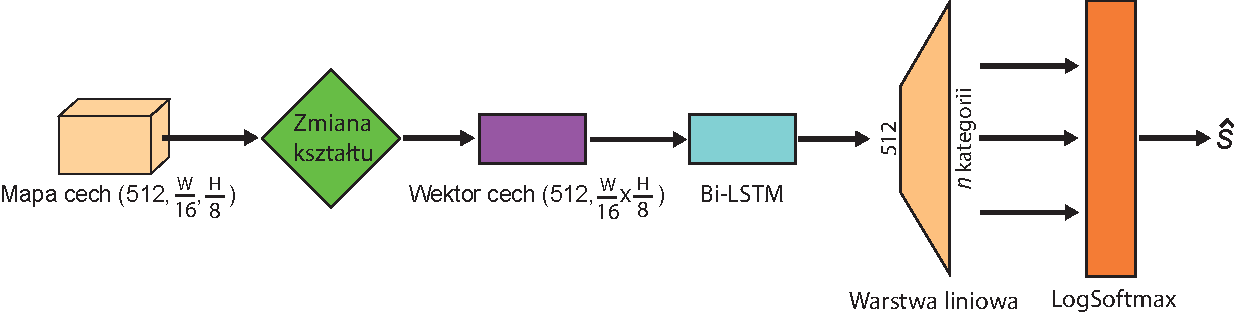
\includegraphics[width=15cm]{images/Decoder_illst}
	\caption{Wizualizacja struktury dekodera modelu uczenia głębokiego.}
	\label{fig:decoder-model-vis}
\end{figure}

Dekoder modelu składa się z~pojedynczej warstwy LSTM z~biblioteki \textit{PyTorch}, inicjalizowanej wielkością wejścia równą $512$, liczbą cech stanu ukrytego równą $256$, określoną dwukierunkowością na~prawdziwą, oraz~argumentem \pyth|batch_first| określającym strukturę tensora wyjściowego jako $(b, s, f)$ zamiast $(s, b, f)$, gdzie~$b$ oznacza serię (ang. \textit{batch}), $s$ sekwencję (ang. \textit{sequence}), zaś $f$ cechy (ang. \textit{feature}).

Warstwa rzutująca mapę otrzymanych cech na~kategorie wyjściowe jest~warstwą liniową\linebreak z~biblioteki \textit{PyTorch}. Jako liczbę cech wejściowych otrzymuje wartość $512$, a~liczba cech wyjściowych określana jest~przez odpowiedni argument konstruktora.

Metoda \pyth|forward()| tej klasy w~pierwszej kolejności pobiera wymiary przekazanego jej tensora do~zmiennych \pyth|b|, \pyth|c|, \pyth|h| oraz~\pyth|w|, na~podstawie których dokonuje przekształcenia tego tensora do~postaci $(b, c, h \times w)$, który to jest~następnie poddawany permutacji, w~której jest~zamieniany miejscami rozmiar wymiaru drugiego i~trzeciego.

Modyfikacje te można rozumieć jako proces konkatenacji regionów par polifonicznych, którego wizualizacja jest~przedstawiona na~rysunku \ref{fig:rowijanie-nut}.


\begin{figure}[h]
	\centering
	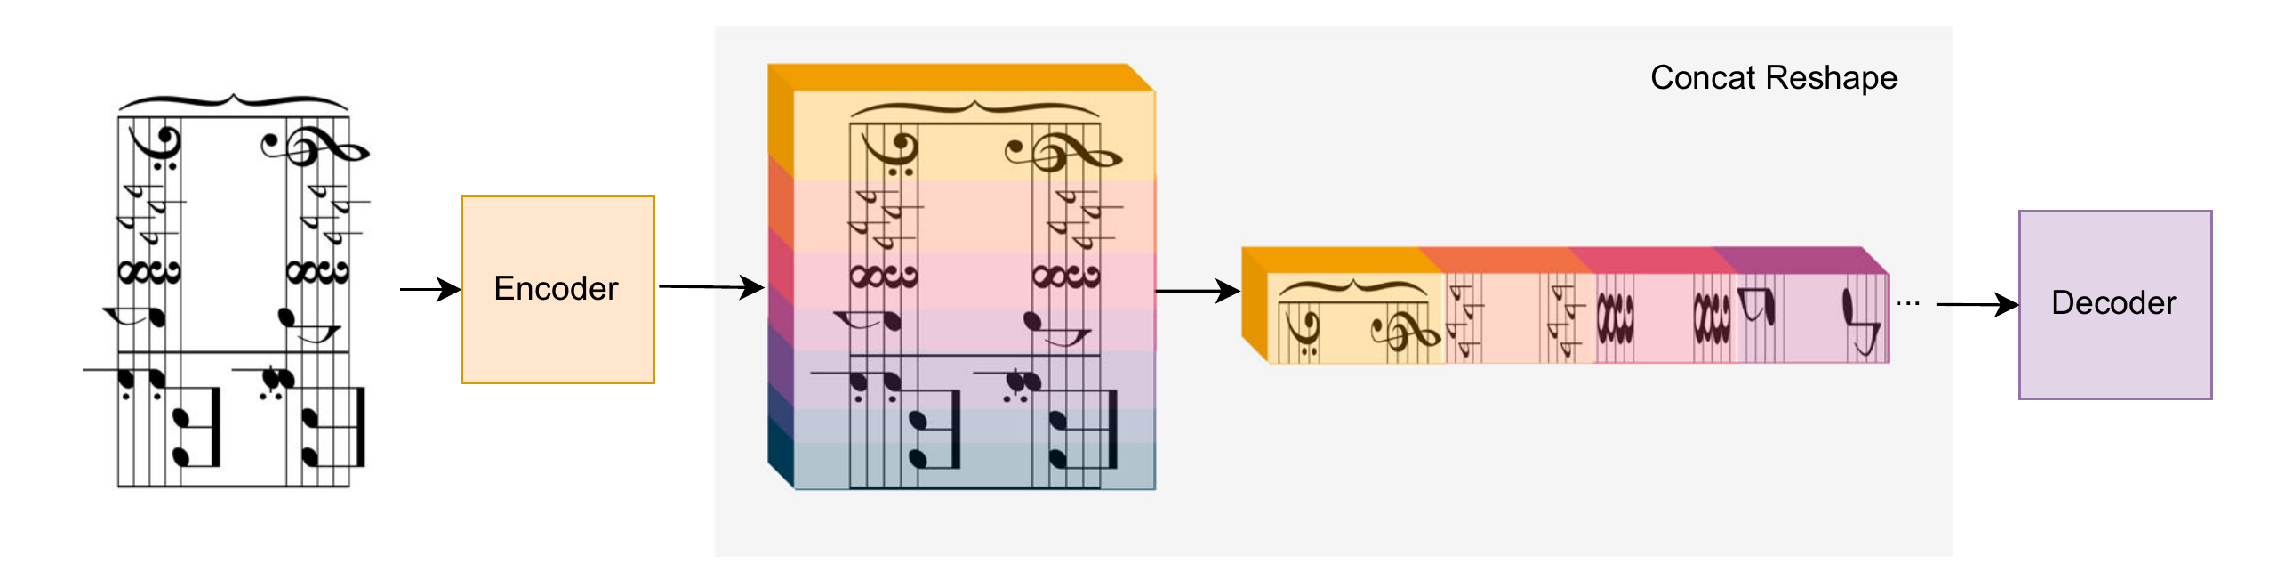
\includegraphics[width=12cm]{images/rozwijanie-nut.png}
	\caption{Wizualizacja procesu konkatenacji regionów par polifonicznych. Źródło: \cite{Rios-Vila2023}}
	\label{fig:rowijanie-nut}
\end{figure}


Pozwala to na~transkrypcję nut w~oryginalnym formacie **kern, gdyż takie ułożenie odpowiada strukturze tego formatu, mianowicie informacje są zapisywane od góry do~dołu i~od lewej do~prawej.

Tak zmodyfikowane dane wejściowe są następnie przekazywane do~warstwy LSTM dekodera, z~którego wyniku działania pobierany jest~wyłącznie wyjściowy tensor, który jest~przekazywany\linebreak do~warstwy liniowej. Rezultat obliczeń warstwy liniowej jest~poddawany permutacji, w~której\linebreak zamieniany ze~sobą są rozmiary wymiarów pierwszego i~drugiego.

Zwracanymi przez dekoder danymi jest~wynik działania funkcji \pyth|log_softmax()|, działającej\linebreak na~trzecim wymiarze wejściowego tensora, która nakłada funkcję softmax, na~którą to nakładany\linebreak jest~logarytm.

\section{Zbiór danych GrandStaff}

Zbiór danych \textit{GrandStaff} jest~pierwszym zbiorem danych zawierającym polifoniczne zapisy\linebreak nutowe na~fortepian, przeznaczonym do~uczenia rozwiązań end-to-end. Jego nazwa odnosi się\linebreak do~angielskiego słowa \textit{grandstaff}, określającego zespół dwóch pięciolinii połączonych klamrą\linebreak na~początku, przeznaczonych do~grania na~fortepianie.

Składa się on z~53882 syntetycznie stworzonych obrazów pojedynczych linii zapisu nutowego na~fortepian, wraz z~ich reprezentacjami w~formatach **kern i~BEKERN oraz~wersjami obrazu przedstawiającymi zniekształcony zapis nutowy.

Format **kern jest~jednym z~najczęściej wykorzystywanych formatów w~komputerowej\linebreak analizie muzyki. Składa się on z~prostego słownika i~prostej do~odczytywania struktury pliku, która jest~po prostu zapisem tekstowym będącym sekwencją linii, gdzie~każda linia jest~złożona z~kolumn\linebreak odseparowanych znakiem tabulacji. Każda z~kolumn zawiera informacje takie jak kodowanie znaków\linebreak zapisu nutowego jak klucze, nuty, pauzy etc. oraz~instrukcje mówiące o~rozpoczęciu czy zakończeniu\linebreak pięciolinii. jest~to zasadniczo tekstowa reprezentacja zapisu nutowego, który został obrócony o~90\degree, którego podobieństwo jest~pokazane na~rysunku \ref{fig:kern-score}. Każda linia pliku **kern jest~czytana od lewej do~prawej, gdzie~symbole są interpretowane w~tym samym czasie, a~następnie od góry do~dołu.

\begin{figure}[htb]
	\centering
	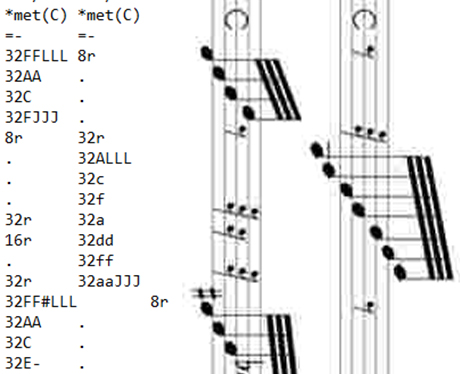
\includegraphics[width=10cm]{images/kern-nuty.jpg}
	\caption{Przykład fragmentu zapisu nutowego w~formacie KERN (lewa) wyrównanego z~wyrenderowanym zapisem nutowym (prawa) ze~zbioru danych GrandStaff.}
	\label{fig:kern-score}
\end{figure}

Dzięki takiej reprezentacji możliwe jest~traktowanie zapisu nutowego w~sposób podobny\linebreak do~normalnego pisma, które składa się z~linii. Pozwala to na~zastosowanie właśnie takich technik\linebreak jak rozwijanie dokumentu\cite{Coquenet2021}, umożliwiając budowę systemów end-to-end dla~polifonicznych\linebreak zapisów nutowych.

\newpage

Dodatkowo w~zbiorze GrandStaff wszystkie zapisy posiadają przetransponowane wersje,\linebreak by możliwe było przygotowanie modelu do~różnie wyglądających zapisów, gdyż w~niektórych\linebreak przypadkach transpozycje zmieniają wygląd i~położenie ogonków i~pałeczek nut, jak jest~to widoczne na~rysunku \ref{fig:score-transposition}.

\begin{figure}[htb]
	\centering
	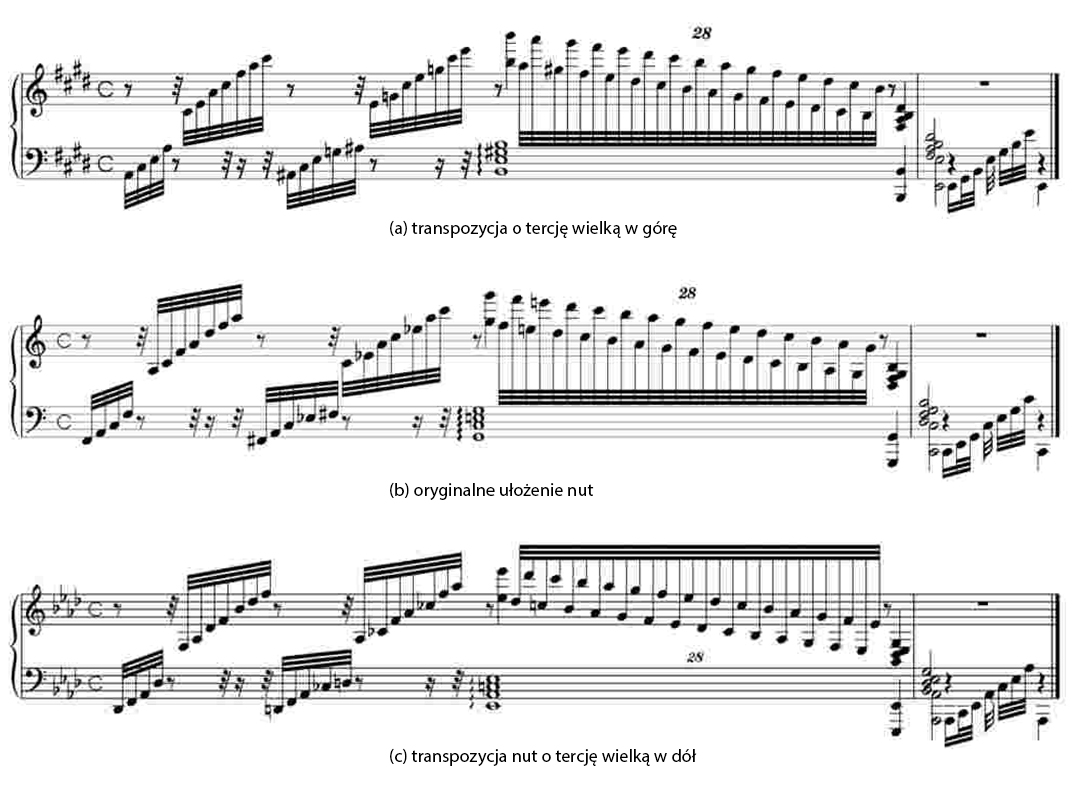
\includegraphics[width=14cm]{images/grandstaff-transpozycje.jpg}
	\caption{Przykład transpozycji zapisu nutowego w~zbiorze danych GrandStaff.}
	\label{fig:score-transposition}
\end{figure}

Kolejną ważną cechą tego zbioru danych jest~posiadanie przez niego zapisu nutowego\linebreak w~wersji nienaruszonej, oraz~zdeformowanej, która stara się naśladować zniekształcenia mogące\linebreak powstać podczas fotografowania czy skanowania, przedstawione na~rysunku \ref{fig:GS-normal-distorted}, określane są przez autorów zbioru jako \textit{Camera GrandStaff}. Pozwala to na~przygotowanie trenowanego modelu\linebreak do~zadania które będzie wykonywał, pozwalając uzyskać mu większą precyzję w~trakcie\linebreak jego wykonywania.

\begin{figure}[htb]
	\centering
	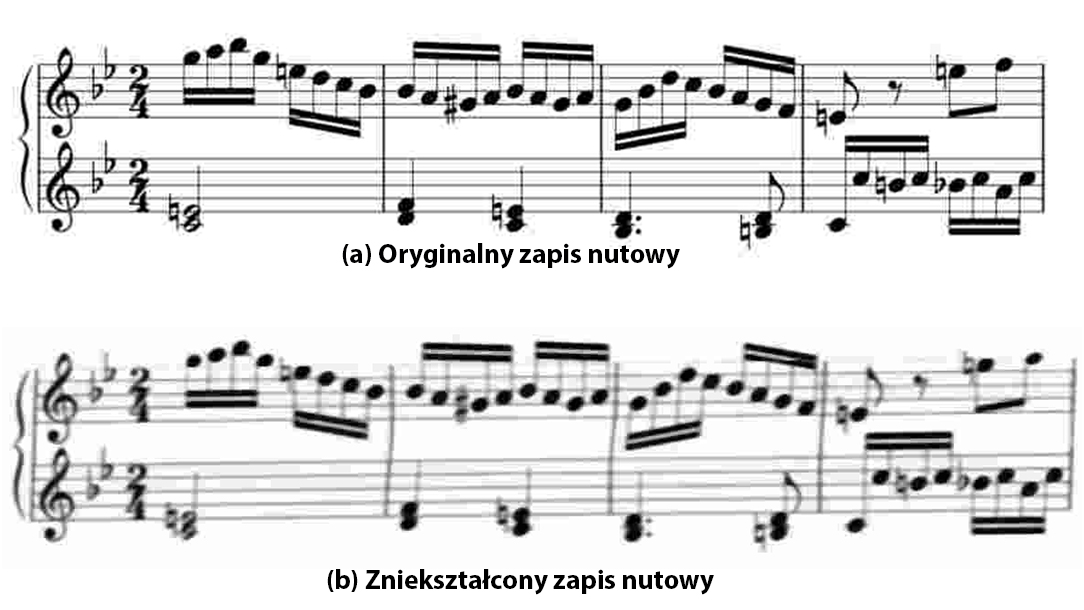
\includegraphics[width=14cm]{images/normal-distorted-GS}
	\caption{Przykład zapisu nutowego ze~zbioru danych GrandStaff w~wersji bez zniekształceń oraz~zniekształconej wersji tego samego zapisu.}
	\label{fig:GS-normal-distorted}
\end{figure}

\section{Trenowanie modelu głębokiego uczenia} \label{ModelTraining}

Trenowanie odbywało się na~platformie \url{vast.ai}, na~zdalnej instancji wyposażonej w~układ\linebreak NVidia GeForce RTX 3090 oraz~103~GB pamięci operacyjnej.

Do wynajętej instancji połączono się z~pomocą SSH, a~następnie zainstalowano na~niej wszystkie niezbędne biblioteki i~programy, które nie były częścią podstawowej konfiguracji kontenera Docker, a~były wymagane do~uczenia modelu. Gdy wszystkie niezbędne wymagania od strony środowiskowej zostały spełnione, przesłano na~instancję pliki z~kodem języka Python, zawierające program uczący model, oraz~spakowany zbiór danych GrandStaff przy pomocy polecenia \pyth|scp|.

Kolejno rozpakowano zbiór danych na~instancji i~utworzono pliki partycjonowania zbioru danych przy pomocy własnego skryptu, gdyż autorzy zbioru takowych plików nie dostarczyli. W~dalszej\linebreak kolejności dostosowano kod programu uczącego do~struktury plików instancji, a~następnie uruchomiono proces uczenia modelu na~zbiorze zniekształconych zapisów nutowych. Najlepsze uzyskane punkty zapisu wytrenowanego modelu pobrano na~lokalny komputer przy pomocy polecenia \pyth|scp|. 

Po zakończeniu trenowania modelu, proces powtórzono, tym razem z~udziałem niezniekształconych zapisów nutowych.

Uzyskano tym sposobem dwa modele, oba trenowane przez 25 epok, pierwszy na~zbiorze Camera GrandStaff, drugi zaś na~zbiorze GrandStaff. Czas uczenia każdego z~modeli wyniósł około 24 godzin.

Podczas trenowania pierwszego modelu wykorzystanie pamięci układu GPU wyniosło około 14~GB, oraz~około 15~GB pamięci operacyjnej, natomiast wykorzystanie pamięci układu GPU wyniosło około 9,4  GB, oraz~około 19~GB pamięci operacyjnej przy trenowaniu modelu drugiego. Pierwszy otrzymany model posiada 20,8 miliona parametrów, drugi zaś 20,6 miliona parametrów.

W testach syntetycznych przeprowadzonych na~odpowiednich testowych podzbiorach zbioru\linebreak danych otrzymane modele osiągnęły wyniki:

\begin{table}[htb]
	\centering
	\begin{tabular}{|c|c|c|}
		\hline
		\ & Model I~& Model II \\
		\hline
		CER & 10,951\% & 6,697\% \\
		SER &  9,178\% & 7,547\% \\
		LER & 28,653\% & 21,14\% \\
		\hline
	\end{tabular}
	\caption{Tabela wyników uzyskanych przez wytrenowane modele. CER - współczynnik błędów znaków (Character Error Rate), SER - współczynnik błędów sekwencji (Sequence Error Rate), LER - współczynnik błędów w~linii (Line Error Rate)}
	\label{models-scores}
\end{table}

Uzyskane wyniki są zbliżone do~tych uzyskanych przez autorów modelu\cite{Rios-Vila2023}.

\subsection{Główna funkcja uczenia modelu}

\begin{lstlisting}[caption={Główna funkcja procesu uczenia modelu.}, label={model-training-main}]
def main(train_path, val_path, test_path, encoding="krn", model_name="CRNN"):
	outpath = f"./out"
	os.makedirs(outpath, exist_ok=True)
	os.makedirs(f"{outpath}/hyp", exist_ok=True)
	os.makedirs(f"{outpath}/gt", exist_ok=True)
	
	train_dataset, val_dataset, test_dataset = load_dataset(train_path, val_path, test_path)
	
	_, i2w = train_dataset.get_dictionaries()
	
	train_dataloader = DataLoader(train_dataset, batch_size=1, num_workers=6, collate_fn=batch_preparation_ctc, shuffle=True)
	val_dataloader = DataLoader(val_dataset, batch_size=1, num_workers=6, collate_fn=batch_preparation_ctc)
	test_dataloader = DataLoader(test_dataset, batch_size=1, num_workers=6, collate_fn=batch_preparation_ctc)
	
	maxheight, maxwidth = train_dataset.get_max_hw()
	
	lightning_model, torch_model = get_model(maxwidth=maxwidth, maxheight=maxheight, in_channels=1, blank_idx=len(i2w), out_size=train_dataset.vocab_size()+1, i2w=i2w, model_name=model_name, output_path=outpath)
	
	wandb_logger = WandbLogger(project='E2E_Pianoform', name=model_name)
	
	early_stopping = EarlyStopping(monitor='val_SER', min_delta=0.01, patience=5, mode="min")
	
	checkpointer = ModelCheckpoint(dirpath=f"./weights/", filename=f"{model_name}", monitor="val_SER", mode='min', save_top_k=3, verbose=True)
	
	trainer = Trainer(max_epochs=25, logger=wandb_logger, callbacks=[checkpointer, early_stopping])
	
	trainer.fit(lightning_model, train_dataloader, val_dataloader)
	
	model = LighntingE2EModelUnfolding.load_from_checkpoint(checkpointer.best_model_path, model=torch_model)
	trainer.test(model, test_dataloader)
	wandb.finish()
\end{lstlisting}

Główna funkcja trenowania modelu pobiera jako argumenty ścieżki do~plików partycjonowania zbioru danych, nazwę typu kodowania informacji oraz~nazwę trenowanego modelu.

Rozpoczyna swoje działanie poprzez utworzenie niezbędnych katalogów, po czym przystępuje do~ładowania zbioru treningowego, walidacyjnego oraz~testowego na~podstawie przekazanych plików partycjonowania. 

Gdy zbiory te zostaną załadowane następuje pozyskanie słowników ze~zbioru do~trenowania, które są niezbędne do~poprawnego pozyskiwania informacji z~obrazów.

Po otrzymaniu słowników tworzone są obiekty \pyth|DataLoader|, zawierające przypisane im zbiory, sampler oraz~iterator po zbiorze danych. Każdy z~tych obiektów ma przypisany rozmiar serii na~$1$, sześć podprocesów zajmujących się ładowaniem  danych, oraz~funkcję zestawiającą dane serii \linebreak na~\pyth|batch_preparation_ctc|, która przygotowuje dane wejściowe do~odpowiedniego formatu. \pyth|train_dataloader| ma dodatkowo określone przetasowanie na~prawdziwe, by ograniczyć\linebreak możliwość nadmiernego dopasowania modelu do~zbioru treningowego, gdyby był okazywany\linebreak modelowi w~tej samej kolejności w~każdej epoce.

Kolejnym ważnym krokiem jest~utworzenie dwóch obiektów modeli, gdzie~\pyth|lightning_model| jest~obiektem biblioteki \textit{Lightning} na~którym wykonywane będzie uczenie, oraz~\pyth|torch_model|, który jest~głównym szkieletem modelu napisanym w~bibliotece \textit{PyTorch}.

Następnie tworzony jest~obiekt loggera z~biblioteki \textit{WandB}, dzięki której zapisywane są dane\linebreak całego procesu uczenia w~chmurze, dając lepszy pogląd na~zachowanie się modelu podczas tej\linebreak operacji. W~dalszej kolejności tworzony jest~obiekt wczesnego zatrzymania, z~określonymi parametrami nadzorowania wartości SER (Sequence Error Rate), minimalną zmianą na~poziomie $0,01$ przez $5$ epok by nastąpiło zatrzymanie procesu.

Później tworzony jest~obiekt klasy \pyth|ModelCheckpoit|, którego zadaniem jest~tworzenie punktów zapisu modelu po każdej epoce, zapisując trzy najlepsze modele według kryterium najmniejszego parametru SER, w~określonym argumentem katalogu.

By umożliwić trenowanie modelu kreowany jest~obiekt klasy \pyth|Trainer|, z~określeniem ile\linebreak maksymalnie epok może pracować, wskazaniem loggera oraz~przekazaniem wcześniej utworzonych obiektów punktów zapisu oraz~wczesnego zatrzymania.

W momencie posiadania wszystkich niezbędnych danych i~obiektów, wywoływana jest~metoda \pyth|fit()| obiektu trenera, której przekazywany jest~model, oraz~moduły ładujące dane zbioru treningowego oraz~walidacyjnego.

Po zakończeniu trenowania modelu, tworzony jest~nowy obiekt modelu na~podstawie\linebreak najlepszego punktu zapisu, który to jest~używany do~przeprowadzenia testu na~zbiorze testowym,\linebreak poprzez wywołanie metody \pyth|test()| obiektu trenera, by ocenić jakoś uzyskanego modelu\linebreak na~wcześniej nie przedstawianych mu danych.